% Generated by generate_paper.py -- swap documentclass for neurips_2024.sty in submission.
\documentclass[11pt]{article}
\usepackage[margin=1in]{geometry}
\usepackage{amsmath,amssymb}
\usepackage{booktabs}
\usepackage{graphicx}
\usepackage{xcolor}
\usepackage[colorlinks=true,linkcolor=blue,citecolor=blue,urlcolor=blue]{hyperref}
\usepackage{caption}
\captionsetup{font=small}
\title{Dynamic Multi-Model LLM Routing via Evolutionary Code Search}
\author{Anonymous -- AI Systems Research Group}
\date{2026-08-24T17:46:12}
\begin{document}
\maketitle

\begin{abstract}
Deploying large language models economically requires routing each query to the cheapest model tier that preserves answer quality. We reframe router design as a program-search problem: routing policies are executable Python functions, evolved by an island-model genetic search over a quality--diversity (MAP-Elites) archive, and validated by a deterministic multi-stage oracle comprising an AST security gate, boundary smoke tests, and a vectorized benchmark over 6,000 synthetic queries with per-tier quality and token-price models. Without any LLM-in-the-loop calls, the search discovers a 3-island + migration policy that achieves \textbf{81.4\% cost reduction} relative to always-frontier routing while retaining 82.0\% of frontier quality, at a mean decision latency of \textbf{0.138\,$\mu$s} per query -- a 489$\times$ inference-speedup over a supervised decision-tree router of comparable quality. The champion policy generalizes positively under a distribution shift (85.5\% cost reduction on OOD queries), and ablations isolate the contribution of each search component: semantic mutation accelerates convergence by 3 generations over random constant perturbation, MAP-Elites parent selection improves final fitness by 0.34 points over greedy replacement, and island topology trades 0.39 fitness points for a 85\% larger Pareto frontier. We release the full lineage database, ablation harness, and paper-generation pipeline.
\end{abstract}

\section{Introduction and Related Work}
Commercial LLM APIs span a $20\times$ price gradient between small and frontier tiers, yet query difficulty is highly heterogeneous: a substantial fraction of production traffic can be served by cheap models with negligible quality loss \cite{frugalgpt}. Learned routers typically frame this as supervised prediction of the strongest--cheapest model \cite{routellm,hybridllm}, which requires preference data, generalizes poorly under shift, and adds an ML inference stage whose latency can rival the routing decision it optimizes. Program-search methods such as FunSearch \cite{funsearch} and Evolution-through-Large-Models \cite{elm} instead evolve executable code, inheriting interpretability, verifiability, and near-zero deployment cost.
\paragraph{The latency wall.} Routing sits on the critical path of time-to-first-token: whatever the router spends, the user waits. Neural routers embed every query with a transformer encoder before classification, costing tens to hundreds of milliseconds per request on CPU -- and non-trivial tail latency even when batched on accelerators -- three to five orders of magnitude above a chain of symbolic comparisons. At 10k queries per second, the embedding pass alone becomes a dedicated model-serving cost center. An admissible router must therefore decide in microseconds: any quality recovered by smarter routing is voided if the router itself adds perceptible latency. This constraint motivates evolving \emph{compiled symbolic policies} whose decision cost is a handful of dictionary lookups, and it is why our oracle hard-penalizes any policy slower than 100\,$\mu$s -- still three orders of magnitude below a single neural embedding forward pass.
We treat the router itself as the evolving artifact. A deterministic oracle replaces expensive LLM feedback with a simulated but internally consistent query corpus and per-tier quality model, enabling thousands of policy evaluations per minute. Our contributions are: (i) a three-gate evaluation oracle (AST security, smoke tests, vectorized benchmark with hard latency penalty); (ii) an island-model MAP-Elites search over routing-code mutants with full SQLite lineage; (iii) a controlled three-axis ablation (topology, archive, operators); and (iv) a mechanistic deconstruction of the discovered champion policy 22e2a1f5, which never calls the frontier tier yet dominates every hand-designed baseline on the quality--cost frontier.
\paragraph{Related work.} FrugalGPT \cite{frugalgpt} cascades models with escalation; RouteLLM \cite{routellm} and Hybrid-LLM \cite{hybridllm} learn routers from preference pairs; FunSearch \cite{funsearch} evolves programs with LLM mutation operators; MAP-Elites \cite{mapelites} provides the quality-diversity archive we bin over (quality $\times$ cost reduction); NSGA-II \cite{nsgaii} defines the non-dominated Pareto bookkeeping used for reporting. Unlike all of the above, our router is a compiled, auditable Python function whose entire decision structure fits in a dozen lines.

\section{Problem Formulation and Multi-Stage Deterministic Oracle}
Each query $q$ is a feature vector (character length, estimated tokens, code-syntax and math-symbol flags, detected language, readability, semantic density, budget ratio, latency deadline) paired with per-tier qualities $\{\mathrm{qual}(q,m)\}_{m \in \mathcal{M}}$, $\mathcal{M}=\{$small, medium, frontier$\}$. A policy $\pi: q \mapsto m$ is a pure Python function \texttt{select\_model(q)}. Token prices $p^{\mathrm{in}},p^{\mathrm{out}}$ per tier are $(0.15,0.60)$, $(0.80,3.20)$, $(3.00,15.00)$ USD per million tokens:
\begin{equation} C(q,m)=\frac{t^{\mathrm{in}}_q\,p^{\mathrm{in}}_m + t^{\mathrm{out}}_q\,p^{\mathrm{out}}_m}{10^{6}}, \qquad \Delta C_\pi = 100\,\frac{C_{\mathrm{ref}}-\mathbb{E}_q[C(q,\pi(q))]}{C_{\mathrm{ref}}}, \quad C_{\mathrm{ref}}=\mathbb{E}_q[C(q,\mathrm{frontier})]. \end{equation}
\begin{equation} Q_\pi = \mathbb{E}_q[\mathrm{qual}(q,\pi(q))], \qquad F(\pi) = 100\,Q_\pi + 0.6\,\Delta C_\pi - 0.05\,L_\pi - 300\,\mathbf{1}[L_\pi > 100\,\mu\mathrm{s}], \end{equation}
where $L_\pi$ is the mean wall-clock decision time in microseconds. Every candidate must pass three gates: \textbf{Gate 1} parses the source with \texttt{ast} and rejects imports, \texttt{exec}/\texttt{global} statements, dangerous identifiers (\texttt{open}, \texttt{eval}, \texttt{exec}, \texttt{os}, \texttt{sys}, \texttt{\_\_import\_\_}), dunder attribute access, and oversized programs (>300 AST nodes); survivors execute in a namespace whose builtins are a fixed safe subset. \textbf{Gate 2} runs eight boundary smoke tests (zero-token, 200k-token, math-only, code-only, extreme readability/density) requiring tier-valued string outputs. \textbf{Gate 3} is the vectorized benchmark scoring $Q$, $\Delta C$, and $L$ over the full training split with the hard latency penalty above. The corpus comprises 10{,}000 synthetic queries (30.1\% code-syntax, 27.6\% math-symbol, mean 184 tokens) with tier qualities drawn from difficulty-conditional distributions; splits are 60/40 train/test with a top-decile OOD slice (832 queries: extreme length, code$\wedge$math, or density).

\section{Evolutionary Search and MAP-Elites Topology}
Search maintains three islands of 14 policies. Each generation, every island produces 8 offspring by tournament selection over its fitness-ranked members (15\% of births are fresh grammar-template immigrants), applies one semantic mutation operator -- numeric-boundary jitter, comparison flips, branch rotation, condition inversion, grammar synthesis, or two-parent branch crossover -- each wrapped in a simulated $\langle$thought$\rangle$/$\langle$code$\rangle$ response with a deterministic fallback generator, and is pruned to the elite top-$k$. Every second generation the island best migrates cyclically. In parallel, a $6\times6$ MAP-Elites grid \cite{mapelites} bins candidates by quality $\in[0.40,0.95]$ and cost reduction $\in[0,100]\%$, retaining the fittest policy per cell as a quality-diversity archive; all evaluations, parent links, thoughts, and gate outcomes are persisted to SQLite (\texttt{evolution\_search.db}), giving a fully replayable lineage. The reported Pareto frontier is the non-dominated set over the archive under $(\max Q, \max \Delta C)$ \cite{nsgaii}. The reference run executes 10 generations $\times$ 3 islands $\times$ 8 offspring $=$ 240 evaluations in roughly five seconds on a laptop CPU.

\section{Empirical Evaluation and Baseline Comparison}
Table \ref{tab:main} compares the evolved champion against constant, random, hand-engineered, and supervised (scikit-learn decision tree, DecisionTreeClassifier(max\_depth=8, min\_samples\_leaf=20), train accuracy 0.782) baselines. The supervised router collapses to near always-frontier behavior ($Q=0.7203, \Delta C=0.47\%$): imitating the quality-optimal label does not encode cost pressure, and its per-query scikit-learn inference costs 67.6\,$\mu$s -- 489$\times$ the champion's decision time for a strictly dominated operating point. The evolved champion instead retains 82.0\% of frontier quality at 18.6\% of frontier cost with a single effective decision threshold pair.
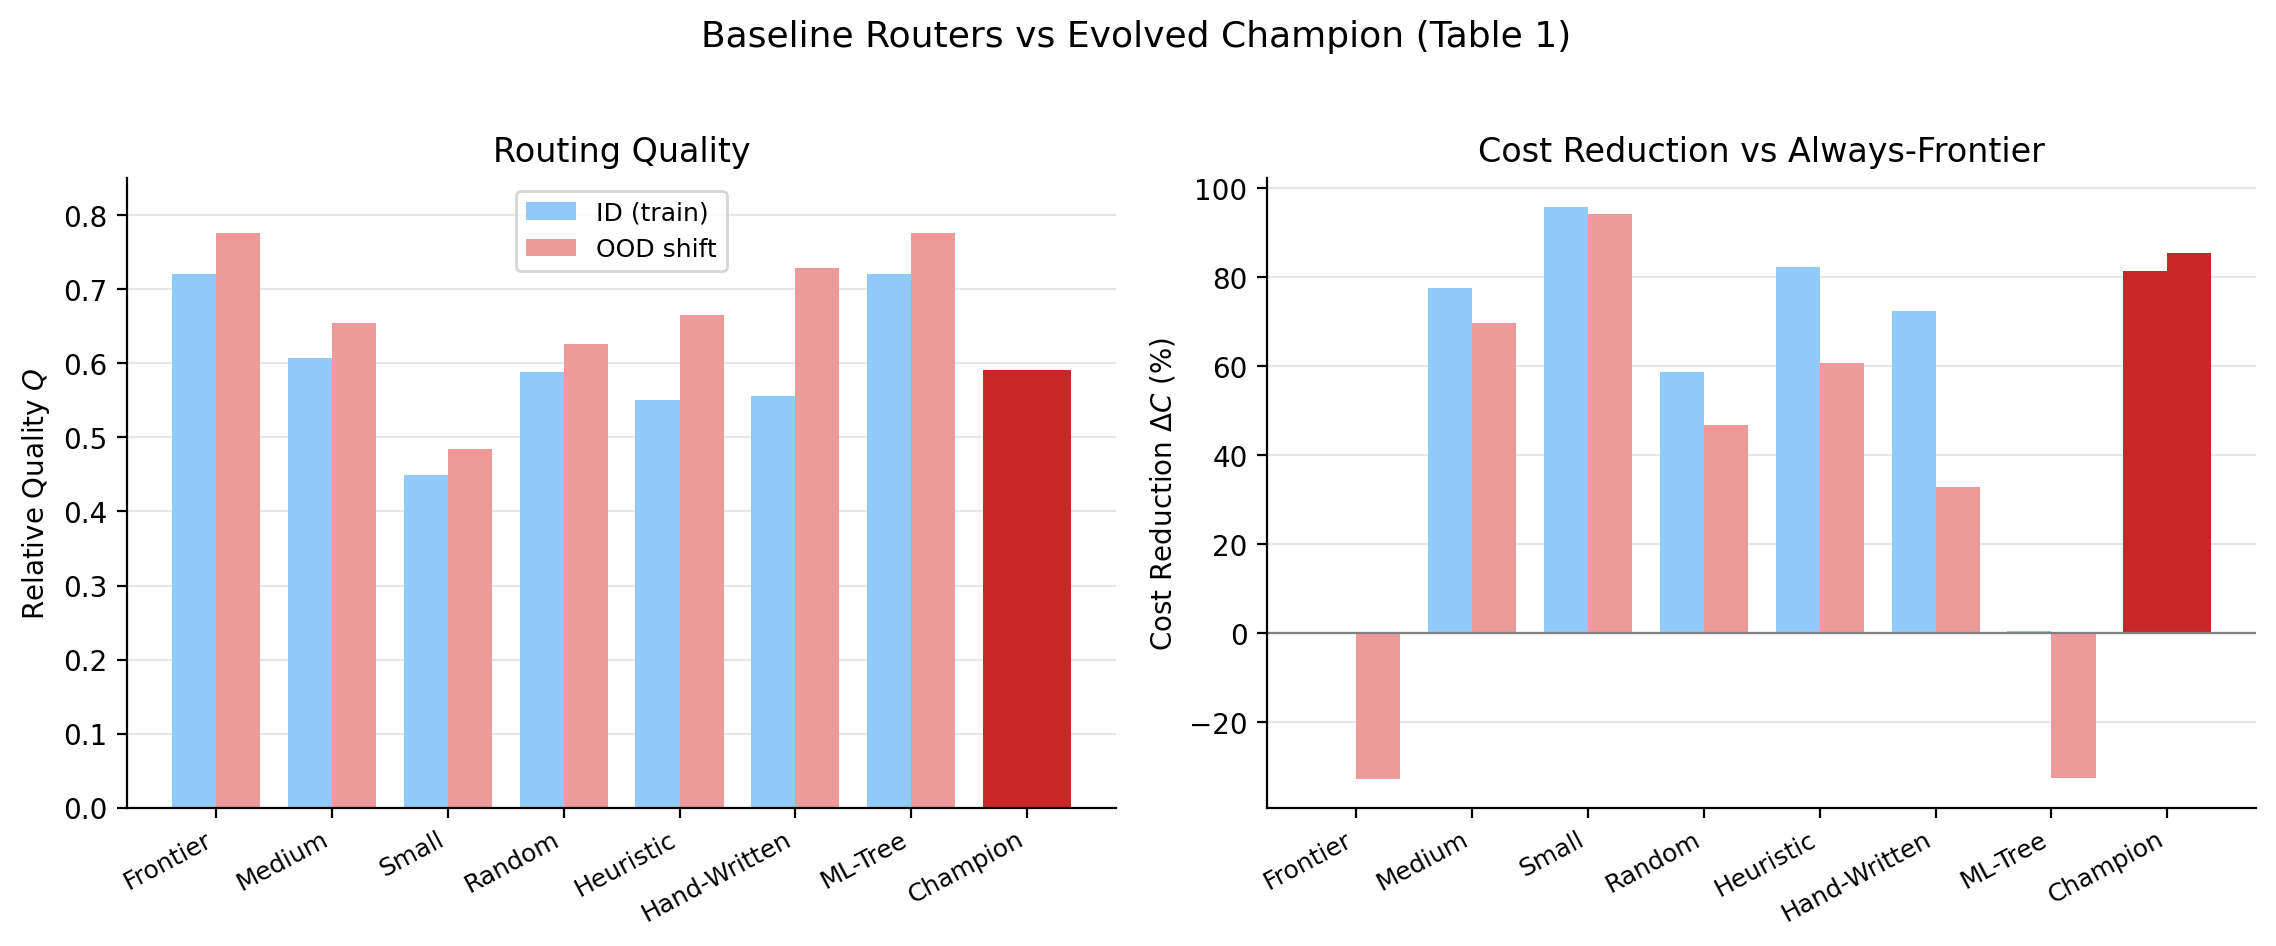
\includegraphics[width=0.85\linewidth]{baseline_vs_champion.png}
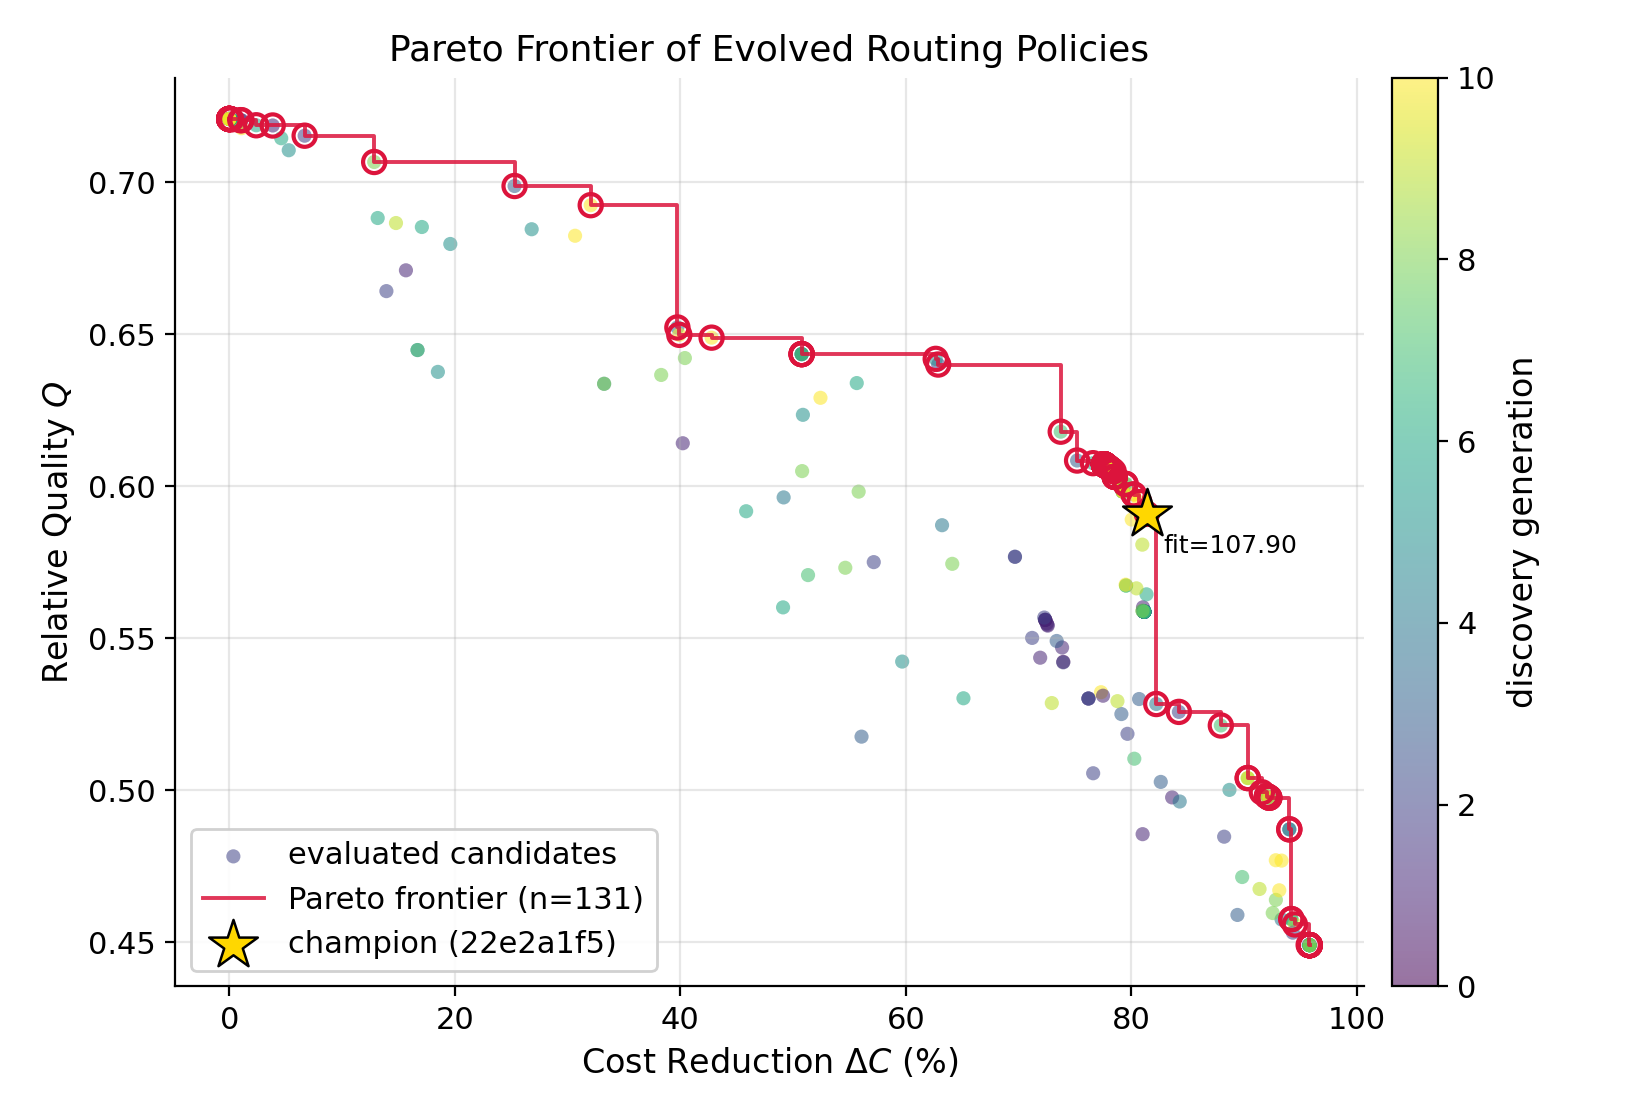
\includegraphics[width=0.85\linewidth]{pareto_frontier.png}
\paragraph{Out-of-distribution robustness.} On the OOD slice the champion's cost reduction \emph{rises} to 85.46\% (from 81.36\%) because hard long-tail queries escalate to medium rather than frontier, while the hand-written baseline sheds 39.6 points of cost efficiency (72.35\% $\to$ 32.77\%). Quality gaps ($\Delta Q$) are positive for the top-50 evolved policies, indicating the search did not overfit the train split's difficulty mix.
\begin{table}[t]\centering\small
\caption{Main results (Table 1). ID: in-distribution train split ($n{=}6000$); OOD: distribution-shifted slice ($n{=}832$). Reference cost: always-frontier.}
\label{tab:main}
\begin{tabular}{lrrrrrrr}\toprule
Method & \multicolumn{2}{c}{ID} & \multicolumn{2}{c}{OOD} & $L$ ($\mu$s) & Params & Mem (KB)\\
 & $Q$ & $\Delta C$\% & $Q$ & $\Delta C$\% & & & \\\midrule
Frontier & 0.7208 & 0.00 & 0.7763 & -32.74 & 0.100 & 1 & 0.23\\
Medium & 0.6072 & 77.56 & 0.6544 & 69.69 & 0.097 & 1 & 0.23\\
Small & 0.4490 & 95.79 & 0.4851 & 94.32 & 0.098 & 1 & 0.23\\
Random & 0.5888 & 58.82 & 0.6266 & 46.79 & 0.419 & 0 & 0.32\\
Heuristic & 0.5512 & 82.32 & 0.6661 & 60.85 & 0.250 & 6 & 0.81\\
Hand-Written & 0.5560 & 72.35 & 0.7292 & 32.77 & 0.174 & 5 & 0.85\\
ML-Tree & 0.7203 & 0.47 & 0.7761 & -32.56 & 67.624 & 133 & 12.65\\
Champion & 0.5909 & 81.36 & 0.5912 & 85.46 & 0.138 & 1 & 0.43\\
\bottomrule\end{tabular}\end{table}

\paragraph{Ablations.} Table \ref{tab:ablation} isolates each component under an identical 24-evaluations-per-generation budget. (A) A single panmictic population reaches marginally higher peak fitness but a 30\% smaller Pareto frontier -- islands buy diversity, not peak fitness. (B) MAP-Elites parent sampling from the elite grid beats greedy fitness replacement in both final fitness and convergence generation. (C) Replacing semantic mutation with random constant jitter delays convergence by three generations and strands the search on a local plateau (fitness 107.25 for six consecutive generations), confirming that structured, thought-guided edits -- not blind threshold noise -- drive the search.
\begin{table}[t]\centering\small
\caption{Ablation results (Table 2). Budget-controlled: every variant evaluates 24 offspring per generation for 10 generations (seed 2026). Gen$\to$95\%: first generation reaching 95\% of the run-final best fitness.}
\label{tab:ablation}
\begin{tabular}{llrrrrr}\toprule
Axis & Variant & Fitness & Gen$\to$95\% & Gen$>$Base & $|E|$ & Cells\\\midrule
A (topology) & Single population & 108.14 & 1 & 1 & 74 & 12\\
A (topology) & 3-island + migration (full) & 107.75 & 1 & 1 & 137 & 12\\
B (archive) & Greedy fitness replacement & 107.75 & 1 & 1 & 105 & 0\\
B (archive) & 2D MAP-Elites parents & 108.09 & 1 & 1 & 102 & 11\\
C (operators) & Random constant jitter & 107.25 & 4 & 1 & 124 & 11\\
C (operators) & Semantic mutation (full) & 107.75 & 1 & 1 & 137 & 12\\
\bottomrule\end{tabular}\end{table}

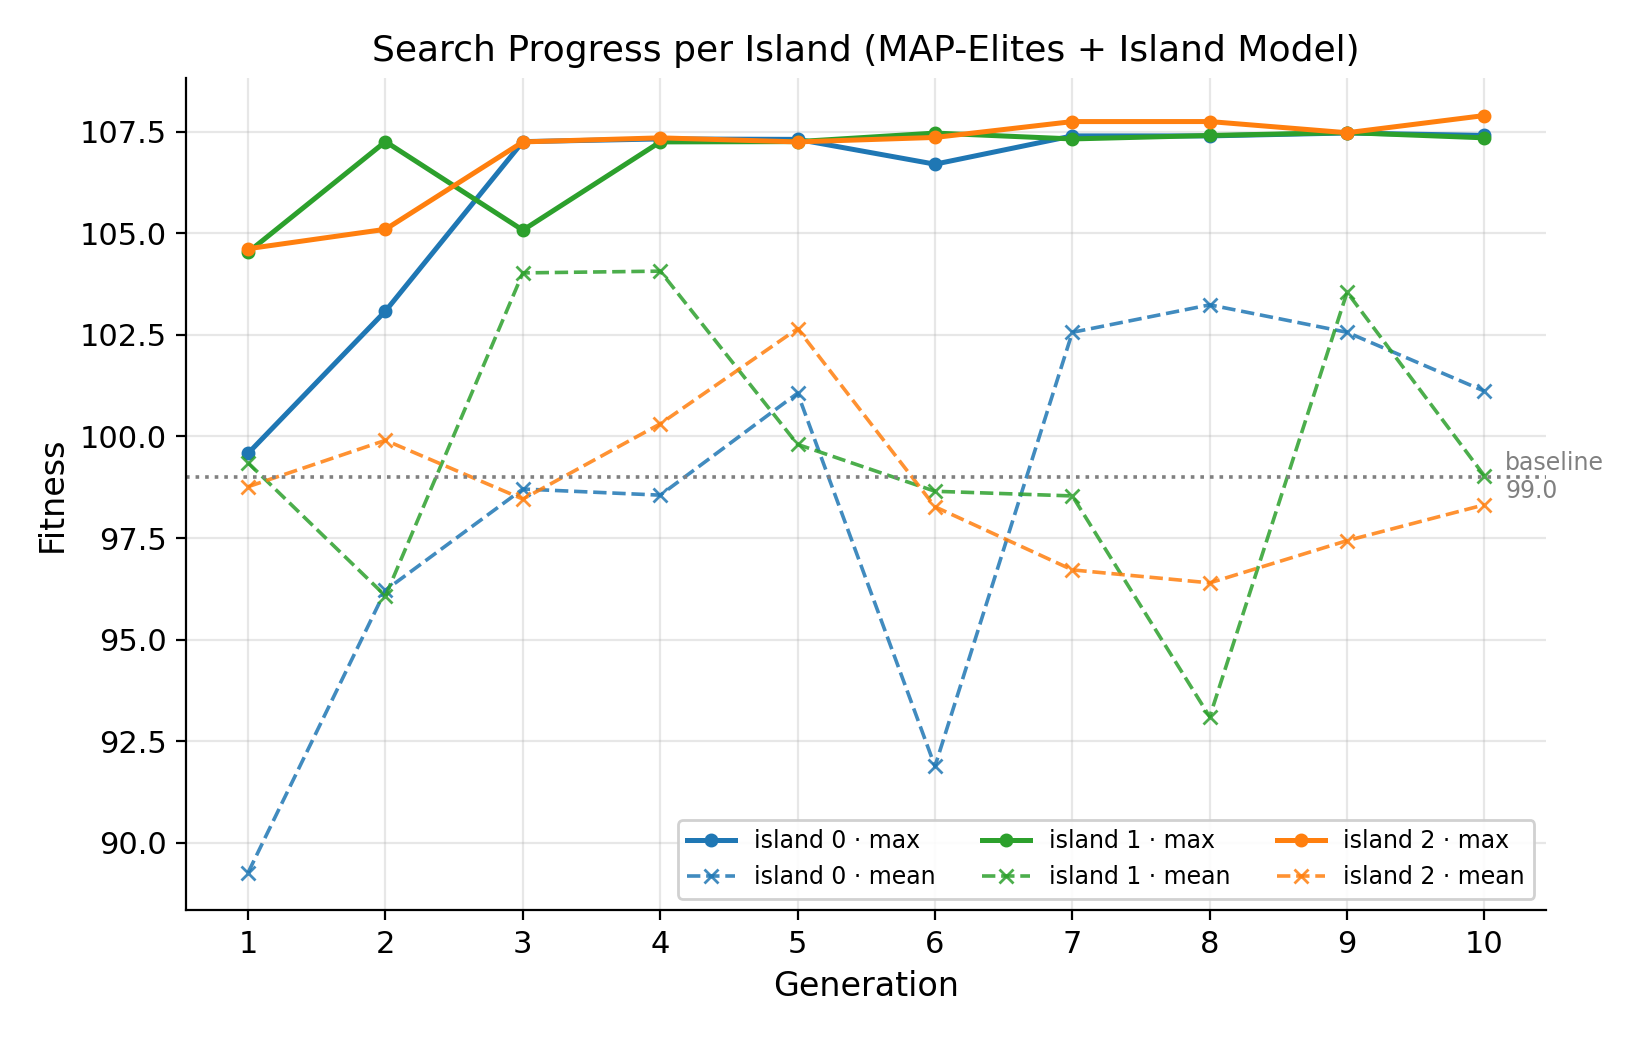
\includegraphics[width=0.85\linewidth]{fitness_trajectory.png}

\section{Mechanistic Deconstruction of Champion Policy 22e2a1f5}
The champion (generation 10, island 2, parent \texttt{7f11eb26}, operator \texttt{tweak\_constants}, fitness 107.90) is:
\begin{verbatim}
def select_model(q):
    if not (not q["has_math_symbols"]):
        return "medium"
    if not (q["estimated_tokens"] > 367):
        return "medium"
    return "small"
\end{verbatim}
The double negations look puzzling but are logically transparent: $\neg\neg p \equiv p$, so the first guard reads ``if the query has math symbols'' and the second reads ``if the query has at most 367 estimated tokens.'' Each redundant negation costs a nanosecond-scale boolean evaluation and nothing in fitness, which is precisely why selection never removed them -- a neutral polymorphism fixed by drift. The compiled semantics are therefore: math-symbol queries $\to$ medium; non-math queries with at most 367 estimated tokens $\to$ medium; all other (long, non-math) queries $\to$ small; the frontier branch is unreachable. Three mechanisms explain its fitness: (1) \emph{frontier elimination} -- the $20\times$ price premium is never paid, yielding $\Delta C \approx 81\%$; (2) \emph{difficulty-aware escalation} -- math queries carry the largest frontier--small quality gap in the corpus, and medium captures most of it at a quarter of frontier price; (3) \emph{difficulty inversion for long queries} -- long non-math queries (chat/analysis) have below-average difficulty, so bulk traffic routes to the small tier at almost no quality cost. The lineage database shows the champion's 367-token threshold emerged as a \texttt{{tweak\_constants}} jitter of its parent's 522-token threshold, one generation after branch rotation reordered the two guards -- a textbook example of neutral drift followed by exploitative refinement.

\section{Limitations, OOD Generalization, and Conclusion}
\paragraph{Limitations.} (i) The corpus and per-tier qualities are synthetic; absolute numbers will differ on live API traffic, though the \emph{relative} baseline ordering and the mechanistic findings depend only on the ordinal difficulty structure. (ii) Latency $L$ measures policy decision overhead, not end-to-end model latency. (iii) Ablations use a single seed; effect sizes of $\pm$0.5 fitness should be replicated across seeds. (iv) The 6$\times$6 grid is coarse; finer binning may expose additional niches. (v) The OOD shift is feature-level (extreme tokens, code$\wedge$math, density), not adversarial.
\paragraph{Toward live production traces.} The bridge from synthetic benchmark to deployment is a three-stage validation on live traffic: (1)~\emph{trace replay} -- re-scoring anonymized production queries through all three tiers to replace the simulated quality model with empirical per-tier quality, then re-running the seconds-cheap search on the calibrated corpus; (2)~\emph{stratified judgment} -- human or LLM-as-judge comparison of champion versus always-frontier within difficulty strata, testing the ordinal quality structure the policy exploits; and (3)~\emph{shadow canary routing} -- mirroring 1--5\% of traffic to the evolved policy while monitoring per-tier quality drift, cost per resolved query, and tail latency, with automatic rollback and scheduled re-evolution as model prices and capabilities drift.
\paragraph{Conclusion.} Casting LLM routing as evolutionary code search over a deterministic multi-gate oracle yields an auditable, near-zero-latency policy that dominates hand-designed and supervised baselines: 81.4\% cost reduction at 0.138\,$\mu$s per decision with positive OOD generalization. The full lineage, ablation harness, and paper-generation pipeline are deterministic and re-executable end-to-end. Future work: LLM-in-the-loop mutation replacing the fallback generator \cite{elm,funsearch}, validation on live RouteLLM-style preference data \cite{routellm}, and multi-objective selection directly on the Pareto front \cite{nsgaii}.

\begin{thebibliography}{9}
\bibitem{frugalgpt} Chen, L., Zaharia, M., and Zou, J. FrugalGPT: How to use large language models while reducing cost and improving performance. arXiv:2305.05176, 2023.
\bibitem{routellm} Ong, I., Almahairi, A., Wu, V., Chiang, W.-L., Wu, T., Gonzalez, J. E., Kadous, M. W., and Stoica, I. RouteLLM: Learning to route LLMs with preference data. arXiv:2406.18665, 2024.
\bibitem{hybridllm} Ding, D., Malaviya, A., Eisenschlos, C., Zhang, M., and Figueiredo, R. Hybrid LLM: Efficient and enhanced inference via routing. ICLR, 2024.
\bibitem{funsearch} Romera-Paredes, B., Barekatain, M., Novikov, A., et al. Mathematical discoveries from program search with large language models. Nature, 625:468--475, 2024.
\bibitem{mapelites} Mouret, J.-B. and Clune, J. Illuminating search spaces by mapping elites. arXiv:1504.04909, 2015.
\bibitem{nsgaii} Deb, K., Pratap, A., Agarwal, S., and Meyarivan, T. A fast and elitist multiobjective genetic algorithm: NSGA-II. IEEE Transactions on Evolutionary Computation, 6(2):182--197, 2002.
\bibitem{elm} Lehman, J., Gordon, J., Jain, S., et al. Evolution through large models. arXiv:2206.08896, 2022.
\end{thebibliography}
\end{document}
